

\subsection{Memory Allocation}

Any model seeking to convert RESOLVE to a lower level representation such as C demands a strategy for handling any memory utilized by the generated code. While dynamic allocation is typically the norm, it is not however the first choice for embedded applications. With the Telos mote constrained to 128 bytes of RAM, developers targeting embedded platforms tend to favor static memory allocation over dynamic, due the memory efficiency it affords. 

%Many programs however benefit greatly from dynamic memory allocation not only in terms of clarity and straightforwardness, but in our case: Accurately modeling exactly what the code being executed is doing. 
%NesC, for example, while giving the illusion of dynamic allocation, behind the scenes actually performs static allocation 

In spite of this, our reasoning for choosing to pursue dynamic allocation over static, rests in the language itself. Being a language that relies heavily on the notion of formally specified objects (components), everything in RESOLVE from the `primitive' types such as booleans and integers, to the more complicated (user defined) ones such as Stacks and Queues, are modeled, specified, and implemented in the same way: Using the standard RESOLVE machinery discussed in Section \ref{sec:specifiying}. 

As such, even the simplest RESOLVE programs still rely heavily on the notion of objects coming and going. Thus, from a verification perspective, creating a tool that allows our translated code to create and destroy such objects in the manner the language itself uses is an important component to capture in formally verified code.

\subsubsection{Allocation using \texttt{salloc}}

The particular allocation scheme that we chose to use is \texttt{salloc()}: A first fit memory allocator. Rather than allocating memory on the heap, \texttt{salloc()} instead uses the stack. At compilation, the allocator provisions a fixed size of memory. It requires a small section of meta-data called a block which contains information of about the size of memory allocated, neighboring blocks, as well if the block is free or not. A sample representation of the stack shown in figure \ref{fig:stack}, is a typical example of allocated memory on the stack.

\begin{figure}[!htb]
\centering
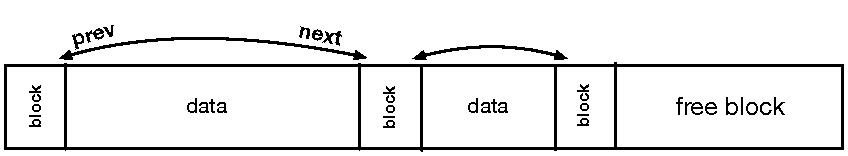
\includegraphics[scale=.55]{figs/stack.pdf}
\caption{Representation of memory stack}
\end{figure}
\label{fig:stack}

\subsubsection{Deallocation using \texttt{sfree}}

A memory allocator must provide a mechanism to release, or free memory in order to indicate that it is not being used and can be reallocated for something else. The \texttt{sfree()} operation is an analogous implementation to the standard C \texttt{free()} function for the stack.

\begin{figure}[!htb]
\centering
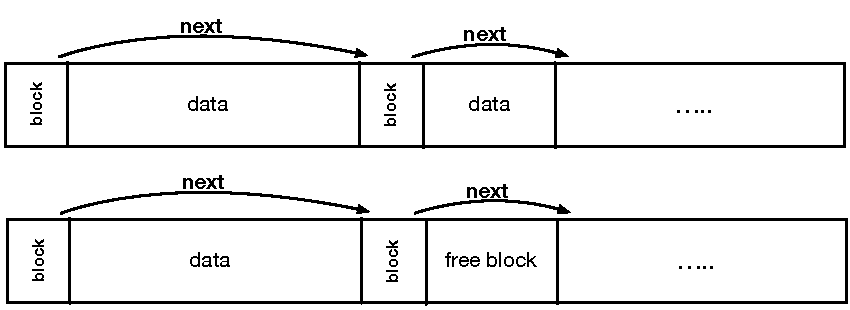
\includegraphics[scale=.55]{figs/sfree.pdf}
\caption{sfree to free memory}
\end{figure}
\label{fig:free}
 
\subsubsection{Optimizations}

A common problem that can occur in memory allocation is fragmentation.  As shown in figure \ref{fig:fragmentation}, fragmentation can lead to inefficient and increased memory usage. This problem is magnified on embedded systems with limited memory capabilities. Simple optimizations can be made however to reduce fragmentation. Splitting is one optimization that \texttt{salloc()} to maximize memory usage. Shown in figure \ref{fig:split}, blocks can be split to the size that is required. Another means of optimizing memory usage is joining together freed blocks. When a call to \texttt{sfree()} is made, neighboring blocks are coalesced together, as shown in figure \ref{fig:fuse}.

\begin{figure}[!htb]
\centering
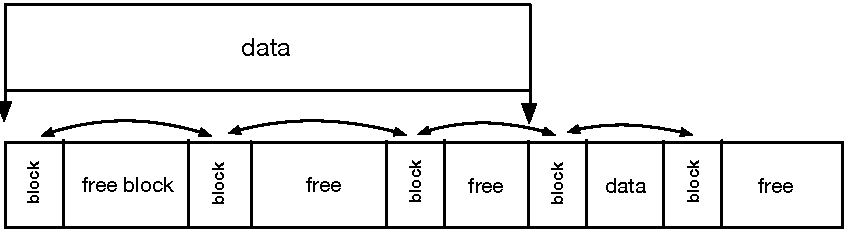
\includegraphics[scale=.55]{figs/fragmentation.pdf}
\caption{fragmentation}
\end{figure}
\label{fig:fragmentation}

\begin{figure}[!htb]
\centering
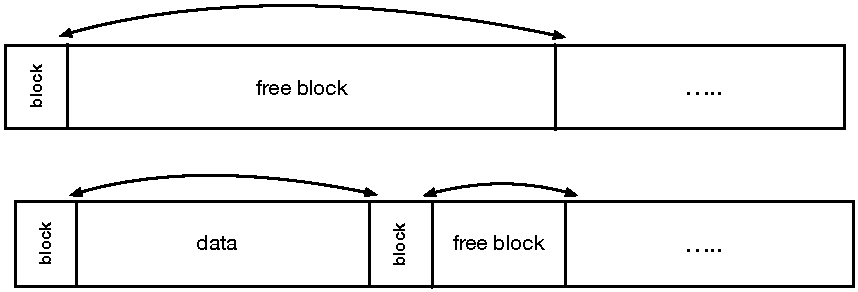
\includegraphics[scale=.55]{figs/split.pdf}
\caption{block splitting}
\end{figure}
\label{fig:split}

\begin{figure}[!htb]
\centering
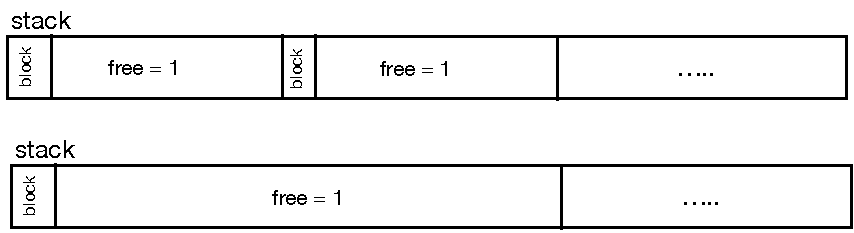
\includegraphics[scale=.55]{figs/fuse.pdf}
\caption{block fusing}
\end{figure}
\label{fig:fuse}
%A stack-based approached to dynamic memory allocation requires a fixed size of memory to be set prior to compilation. 
%To date there have been very few practical applications of verifiable code on physical media. 

\subsection{An LED Implementation}

\begin{verbatim}
void LED_Telos_create() {
		Std_Boolean_Fac_create();
		Std_Integer_Fac_create();
		Std_Clock_Fac_create();
		r_type_ptr __arg_0 = Std_Integer_Fac_Var.core->createFromInteger(4, Std_Integer_Fac_Var.core->Integer);
		LED_Telos_Facility_Var.core = new_Std_LED_Realiz_for_Leds_Template(__arg_0);
		LED_Telos_Facility_Var.Toggling_Capability = new_Toggling_Capability_of_Leds_Template(LED_Telos_Facility_Var.core);
		Std_Integer_Fac_Var.core->Integer->destroy(__arg_0, Std_Integer_Fac_Var.core->Integer);
}
\end{verbatim}